\insertmeeting 
	{Awesome Assembly} 
	{11/04/22}
	{Hagerty High School}
	{Jensen, Jorge, Karissa, Laura, Nathan, Ritam, Robert, Samantha}
	{Images/RobotPics/robot.jpg}
	{4:30 - 7:30}
	
\hhscommittee{Hardware}
\noindent\hfil\rule{\textwidth}{.4pt}\hfil
\subsubsection*{Goals}
\begin{itemize}
    \item Discuss drivetrain

\end{itemize} 

\noindent\hfil\rule{\textwidth}{.4pt}\hfil

\subsubsection*{Accomplishments}
After waiting a while for our poles to arrive and our end connectors to be 3D printed at UCF, we finally got everything we needed to finish assembly of our robot. Our drivetrain was already assembled, we spent a night at UCF doing that when we got our drivetrain printed. All that was left was to get the poles mounted.

However, during early testing, we realized that the robot's wheels were not properly assembled. This was a somewhat time consuming setback, as the wheels weren't intended to be reassembled multiple times, so assembly and disassembly took a while. Once we were finished with that, we were onto the poles.

The poles consist of two pole bases, an 11 inch pole, two 8 inch poles, pole connectors, and a t-brace at the top for stabilization and safety. The 11 inch pole is mounted directly on the robot. A stretchy chord is strewn through the 8 inch poles, and they are bent and held down by a servo to fit within the 18 cubed inch limit. When a match starts, we move the servo to release the poles, putting them in place for the cart holding the grabber to ride up and down it using a pulley system.
We got the pole bases on fine, and the pole connectors were glued on effectively, but an issue arose when getting the poles hooked up. The pole connectors were 3D printed at a team member's house, which we thought would be fine, but when under the stress of the chord, the material was too weak and it would snap. There was no way to fix this without reprinting them, and with the first meet tomorrow, there was no way of doing that in time. We had a drive train, but all we could do now was drive and push cones. Therefore, we had to function as a push bot in the meet.

Our robot wouldn't make for an effective push bot on it's own. The front is a convex trapezoid-like shape, so any attempt to turn while pushing a cone would flop, so we needed a funnel. Lucky for us, we had the materials to make one. Using OnShape, the CAD software we use for our robot, we created a flat funnel that we laser cut on a plank of wood using a GlowForge we have in our room. Using the screw holes made for the pole bases, we had a funnel attached to the robot for tomorrow.
The assembly didn't go exactly how we planned, but we managed to find a way to adapt and do somewhat well in the upcoming meet. We might not be walking in tomorrow feeling completely peachy, but we have a robot with an effective drive train and a good funnel. With the right strategy and a bit of luck, we might be able to get a decent enough rank to work our way up to a great one.

\begin{figure}[htp]
\centering
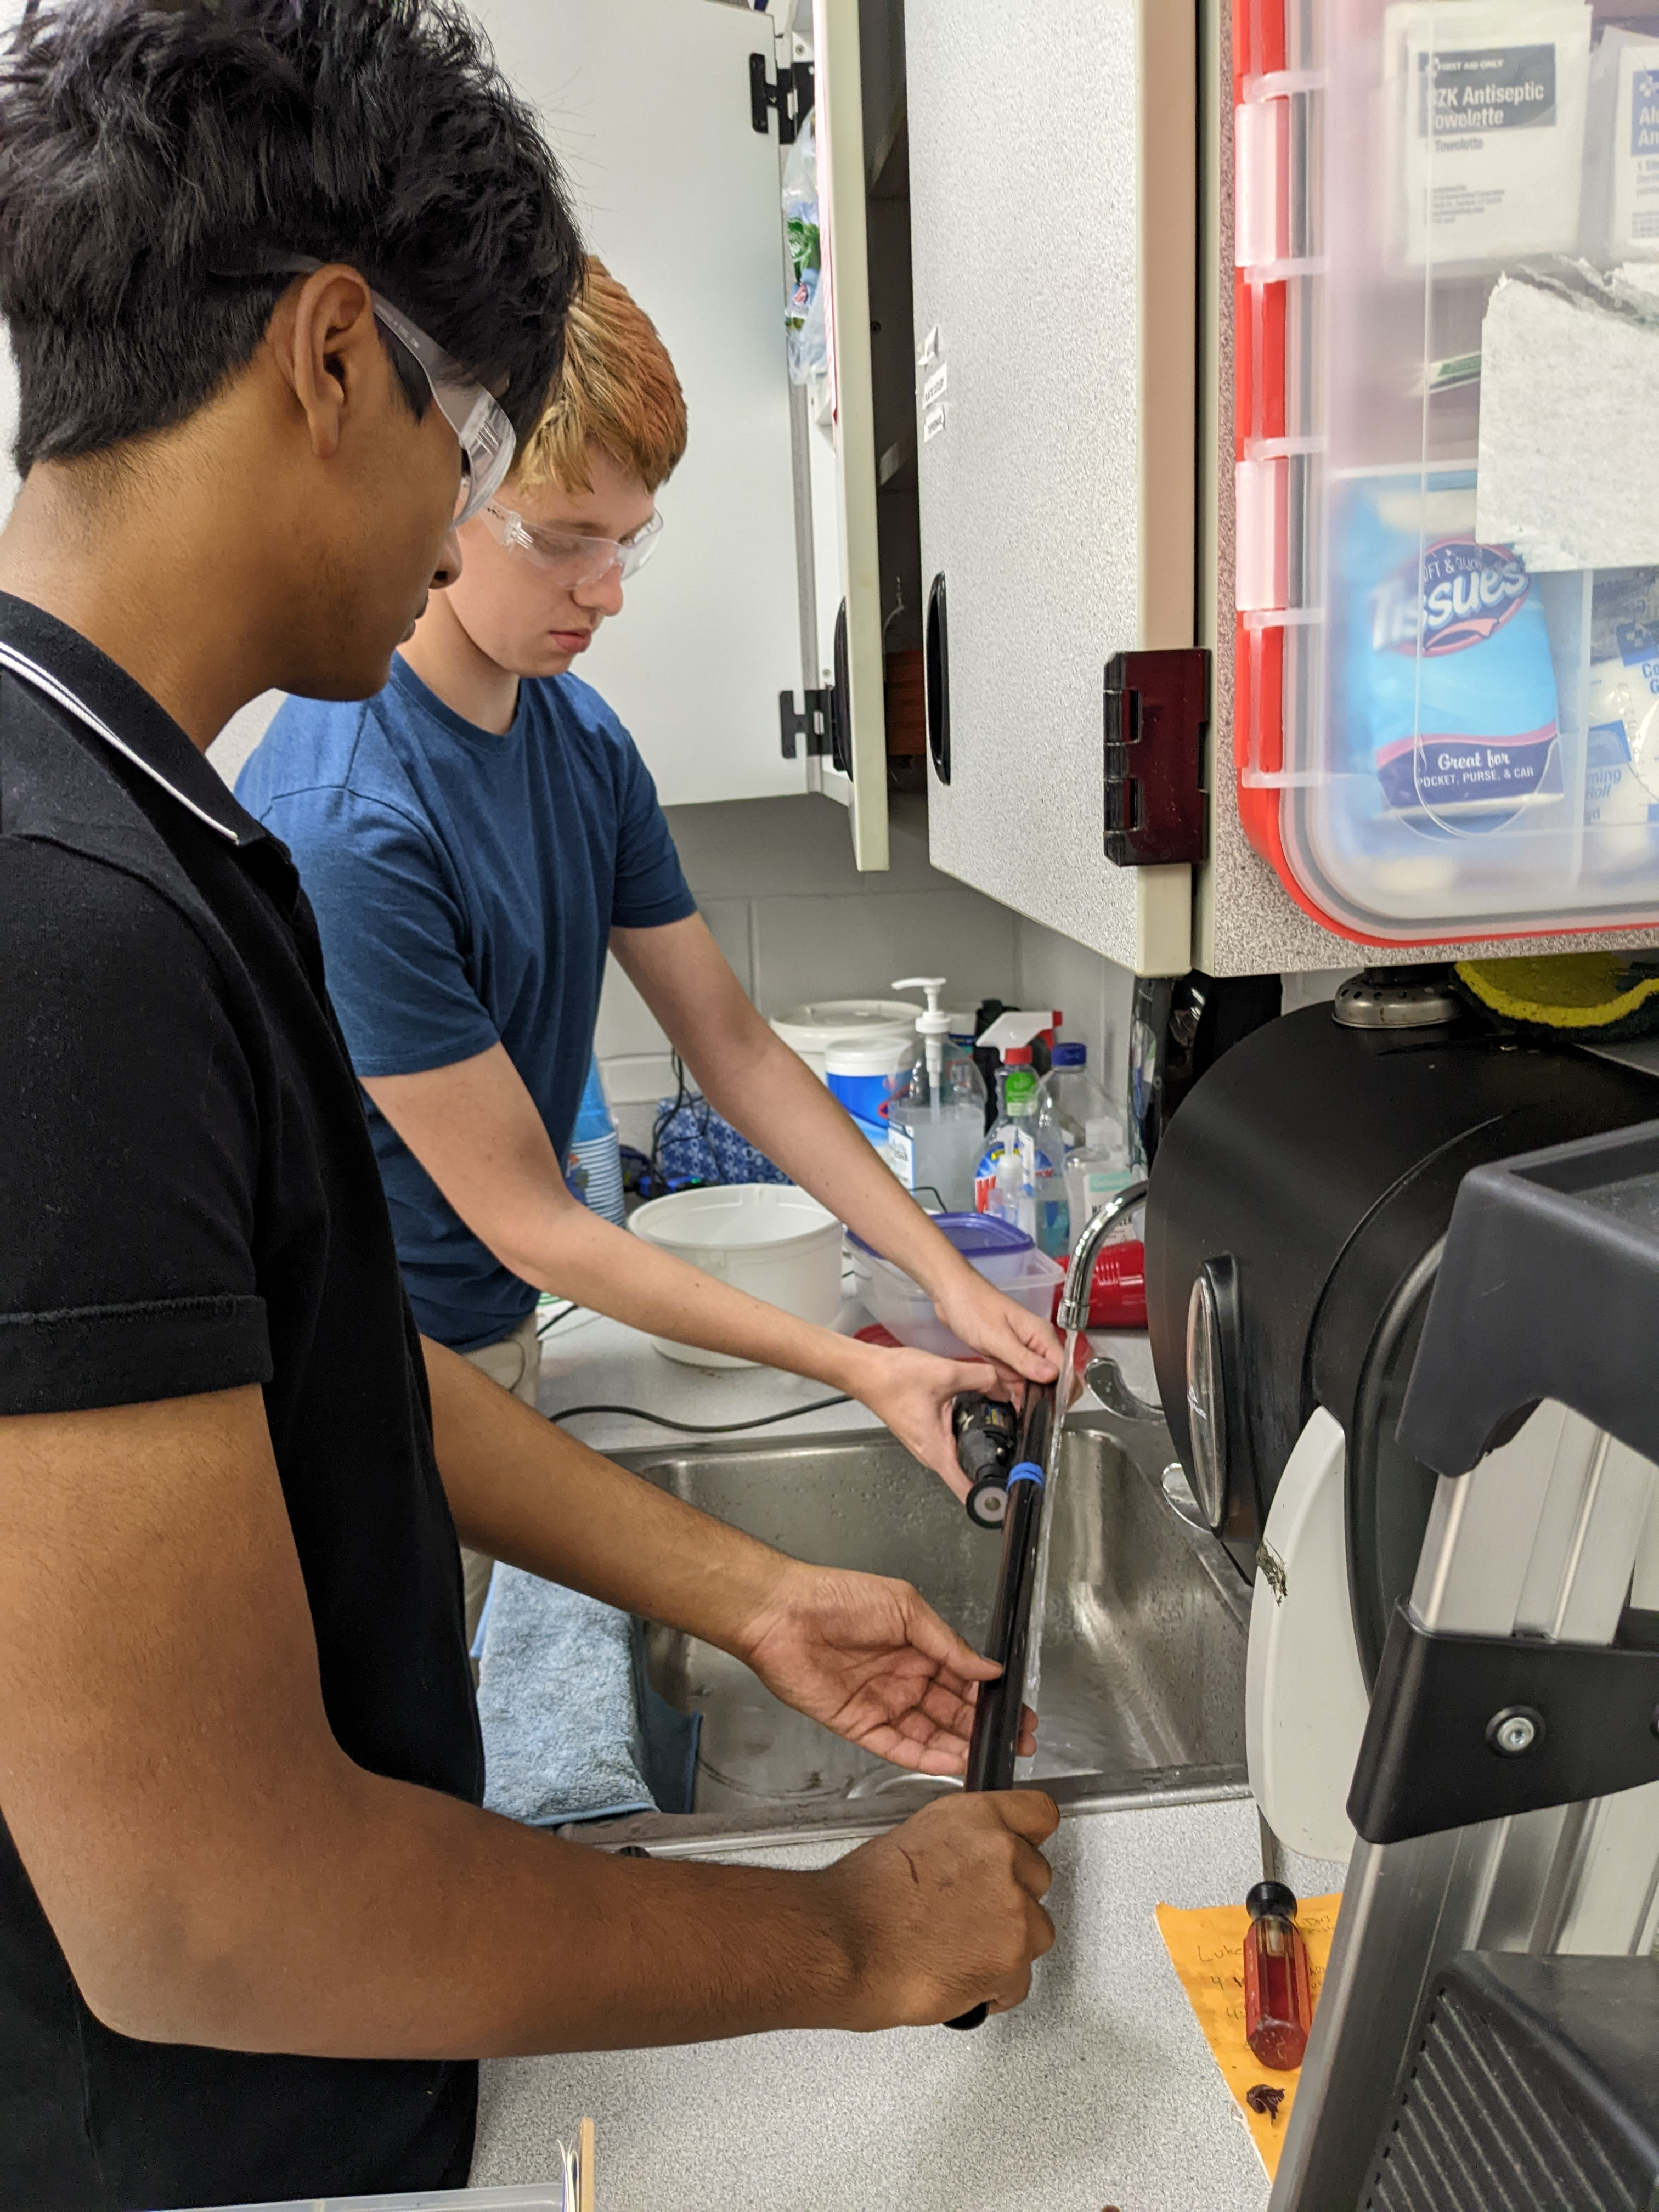
\includegraphics[width=0.9\textwidth, angle=0]{Meetings/November/11-04-22/11-04-22-Poles.jpg}
\caption{Drive path.}
\label{fig:102722_1}
\end{figure}

\whatsnext{
\begin{itemize}
    \item Prepare for meet one
    
\end{itemize} 
}
